%----------------------------------------------------------------------------------------
%	PACKAGES AND OTHER DOCUMENT CONFIGURATIONS
%----------------------------------------------------------------------------------------

\documentclass{article}

\usepackage{fancyhdr} % Required for custom headers
\usepackage{lastpage} % Required to determine the last page for the footer
\usepackage{extramarks} % Required for headers and footers
\usepackage[usenames,dvipsnames]{color} % Required for custom colors
\usepackage{graphicx} % Required to insert images
\usepackage{listings} % Required for insertion of code
\usepackage{courier} % Required for the courier font
\usepackage{lipsum} % Used for inserting dummy 'Lorem ipsum' text into the template
\usepackage{amsmath} % Required for align
\usepackage{enumerate} % Enumerate
\usepackage{amsfonts}
\DeclareMathOperator{\Ima}{im}

% Margins
\topmargin=-0.45in
\evensidemargin=0in
\oddsidemargin=0in
\textwidth=6.5in
\textheight=9.0in
\headsep=0.25in

\linespread{1.1} % Line spacing

% Set up the header and footer
\pagestyle{fancy}
\lhead{\hmwkAuthorName} % Top left header
\chead{\hmwkClass\ (\hmwkClassInstructor): \hmwkTitle} % Top center head
\rhead{\firstxmark} % Top right header
\lfoot{\lastxmark} % Bottom left footer
\cfoot{} % Bottom center footer
\rfoot{Page\ \thepage\ of\ \protect\pageref{LastPage}} % Bottom right footer
\renewcommand\headrulewidth{0.4pt} % Size of the header rule
\renewcommand\footrulewidth{0.4pt} % Size of the footer rule

\setlength\parindent{0pt} % Removes all indentation from paragraphs

%----------------------------------------------------------------------------------------
%	CODE INCLUSION CONFIGURATION
%----------------------------------------------------------------------------------------

\definecolor{MyDarkGreen}{rgb}{0.0,0.4,0.0} % This is the color used for comments
\lstloadlanguages{Perl} % Load Perl syntax for listings, for a list of other languages supported see: ftp://ftp.tex.ac.uk/tex-archive/macros/latex/contrib/listings/listings.pdf
\lstset{language=Perl, % Use Perl in this example
  frame=single, % Single frame around code
  basicstyle=\small\ttfamily, % Use small true type font
  keywordstyle=[1]\color{Blue}\bf, % Perl functions bold and blue
  keywordstyle=[2]\color{Purple}, % Perl function arguments purple
  keywordstyle=[3]\color{Blue}\underbar, % Custom functions underlined and blue
  identifierstyle=, % Nothing special about identifiers                                         
  commentstyle=\usefont{T1}{pcr}{m}{sl}\color{MyDarkGreen}\small, % Comments small dark green courier font
  stringstyle=\color{Purple}, % Strings are purple
  showstringspaces=false, % Don't put marks in string spaces
  tabsize=5, % 5 spaces per tab
        %
        % Put standard Perl functions not included in the default language here
  morekeywords={rand},
        %
        % Put Perl function parameters here
  morekeywords=[2]{on, off, interp},
        %
        % Put user defined functions here
  morekeywords=[3]{test},
        %
  morecomment=[l][\color{Blue}]{...}, % Line continuation (...) like blue comment
  numbers=left, % Line numbers on left
  firstnumber=1, % Line numbers start with line 1
  numberstyle=\tiny\color{Blue}, % Line numbers are blue and small
  stepnumber=5 % Line numbers go in steps of 5
}


%----------------------------------------------------------------------------------------
%	DOCUMENT STRUCTURE COMMANDS
%	Skip this unless you know what you're doing
%----------------------------------------------------------------------------------------

% Header and footer for when a page split occurs within a problem environment
\newcommand{\enterProblemHeader}[1]{
  \nobreak\extramarks{#1}{#1 continued on next page\ldots}\nobreak
  \nobreak\extramarks{#1 (continued)}{#1 continued on next page\ldots}\nobreak
}

% Header and footer for when a page split occurs between problem environments
\newcommand{\exitProblemHeader}[1]{
  \nobreak\extramarks{#1 (continued)}{#1 continued on next page\ldots}\nobreak
  \nobreak\extramarks{#1}{}\nobreak
}

\setcounter{secnumdepth}{0} % Removes default section numbers
\newcounter{homeworkProblemCounter} % Creates a counter to keep track of the number of problems

\newcommand{\homeworkProblemName}{}
\newenvironment{homeworkProblem}[1][Problem \arabic{homeworkProblemCounter}]{ % Makes a new environment called homeworkProblem which takes 1 argument (custom name) but the default is "Problem #"
  \stepcounter{homeworkProblemCounter} % Increase counter for number of problems
  \renewcommand{\homeworkProblemName}{#1} % Assign \homeworkProblemName the name of the problem
  \section{\homeworkProblemName} % Make a section in the document with the custom problem count
  \enterProblemHeader{\homeworkProblemName} % Header and footer within the environment
}{
  \exitProblemHeader{\homeworkProblemName} % Header and footer after the environment
}

\newcommand{\problemAnswer}[1]{ % Defines the problem answer command with the content as the only argument
  \noindent\framebox[\columnwidth][c]{\begin{minipage}{0.98\columnwidth}#1\end{minipage}} % Makes the box around the problem answer and puts the content inside
}

\newcommand{\homeworkSectionName}{}
\newenvironment{homeworkSection}[1]{ % New environment for sections within homework problems, takes 1 argument - the name of the section
  \renewcommand{\homeworkSectionName}{#1} % Assign \homeworkSectionName to the name of the section from the environment argument
  \subsection{\homeworkSectionName} % Make a subsection with the custom name of the subsection
  \enterProblemHeader{\homeworkProblemName\ [\homeworkSectionName]} % Header and footer within the environment
}{
  \enterProblemHeader{\homeworkProblemName} % Header and footer after the environment
}

%----------------------------------------------------------------------------------------
%	NAME AND CLASS SECTION
%----------------------------------------------------------------------------------------

\newcommand{\hmwkTitle}{HW 1} % Assignment title
\newcommand{\hmwkDueDate}{Monday,\ January\ 1,\ 2012} % Due date
\newcommand{\hmwkClass}{CS 5220} % Course/class
\newcommand{\hmwkClassTime}{} % Class/lecture time
\newcommand{\hmwkClassInstructor}{Bindel} % Teacher/lecturer
\newcommand{\hmwkAuthorName}{Nicholas Booher, Shuai \\Jiang, Sepehr Saroukhani} % Your name

% Listings 
\usepackage{listings}
\usepackage{color}

\definecolor{dkgreen}{rgb}{0,0.6,0}
\definecolor{gray}{rgb}{0.5,0.5,0.5}
\definecolor{mauve}{rgb}{0.58,0,0.82}

\lstset{frame=tb,
  language=C,
  aboveskip=3mm,
  belowskip=3mm,
  showstringspaces=false,
  columns=flexible,
  basicstyle={\small\ttfamily},
  numbers=none,
  numberstyle=\tiny\color{gray},
  keywordstyle=\color{blue},
  commentstyle=\color{dkgreen},
  stringstyle=\color{mauve},
  breaklines=true,
  breakatwhitespace=true
  tabsize=3
}



%----------------------------------------------------------------------------------------

\begin{document}
  Our first step to optimizing the program was to jump directly into SSE by using the example script already written in Bitbucket.
  The hope was that the SSE code was a fast enough kernel that we can build a good multiplier around it; indeed, it an immediate
  speed-up was noticed! It approximately doubled our naive multiplication. See figure~\ref{fig:initial}.

  \begin{figure}[h]
    \centering
    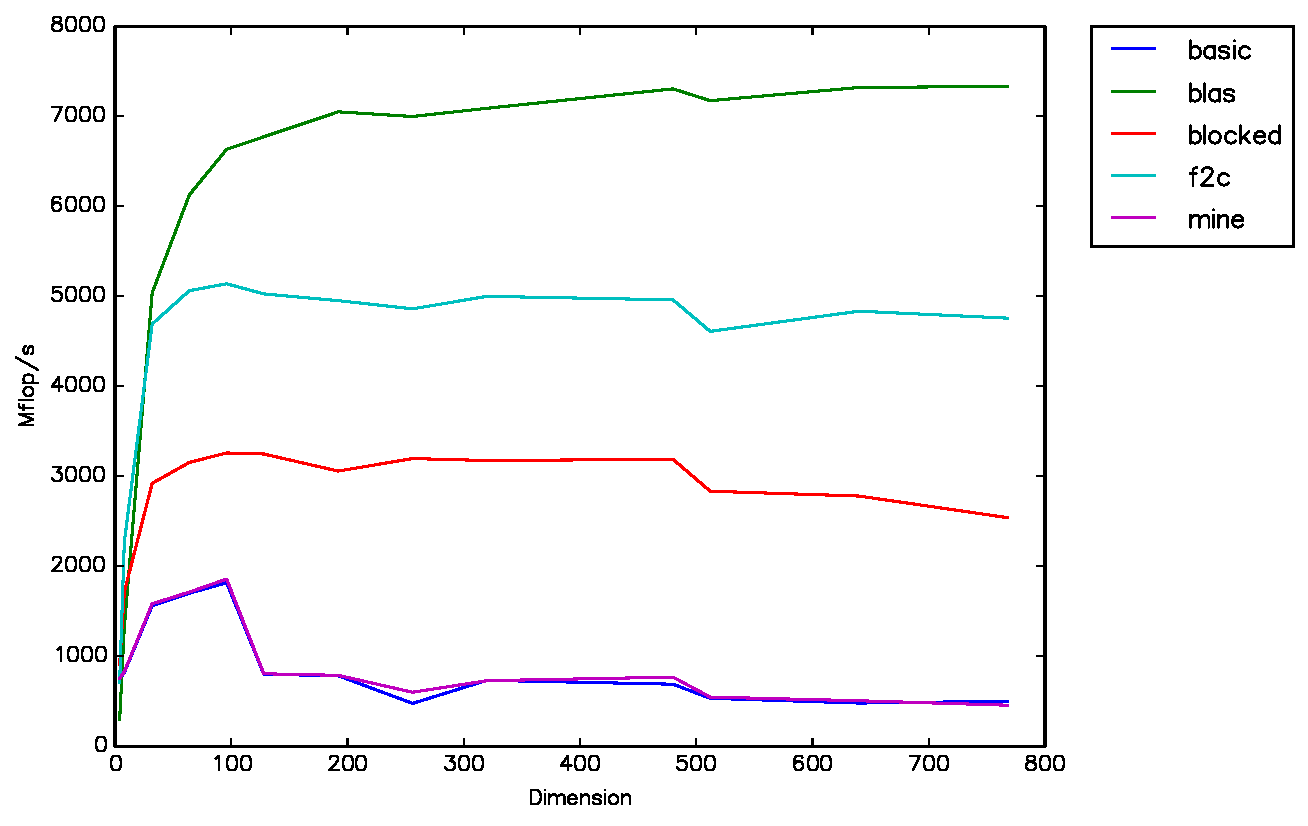
\includegraphics[width=.7\textwidth]{initial.pdf}
    \caption{Our initial set-up using the SSE code provided. Note that the ``blocked'' line is actually our matrix multiply as it was a fairly early version of the code.}
    \label{fig:initial}
  \end{figure}

  What the code does is fairly basic:
  \begin{enumerate}
    \item Intialize arrays At, Bt.
    \item Takes in matrix A, B and copies them into At, Bt such that we have memory layout of 2 by P blocks in A and P by 2 blocks in B.
    \item Loop over the blocks in A and B and multiply, adding the 2 by 2 matrix from the output into the C matrix.
  \end{enumerate}

  We originally compiled this SSE code via the Intel compiler, but weirdly we found that compiling it with the GCC compiler results in a roughly
  33\% speedup over the Intel compiler! We're actually not sure why, but various flags of the ICC doesn't seem to coax the same performance
  out of the code.

  This was all tested on even sizes intially, as there was no need to pad the matrices with anything. The odd cases
  are handled in the natural way, which was to pad a row and column and take the slight hit to the performance.
  When implemented, our performance was still pretty decent. See figure~\ref{fig:odd}.

  \begin{figure}[h]
    \centering
    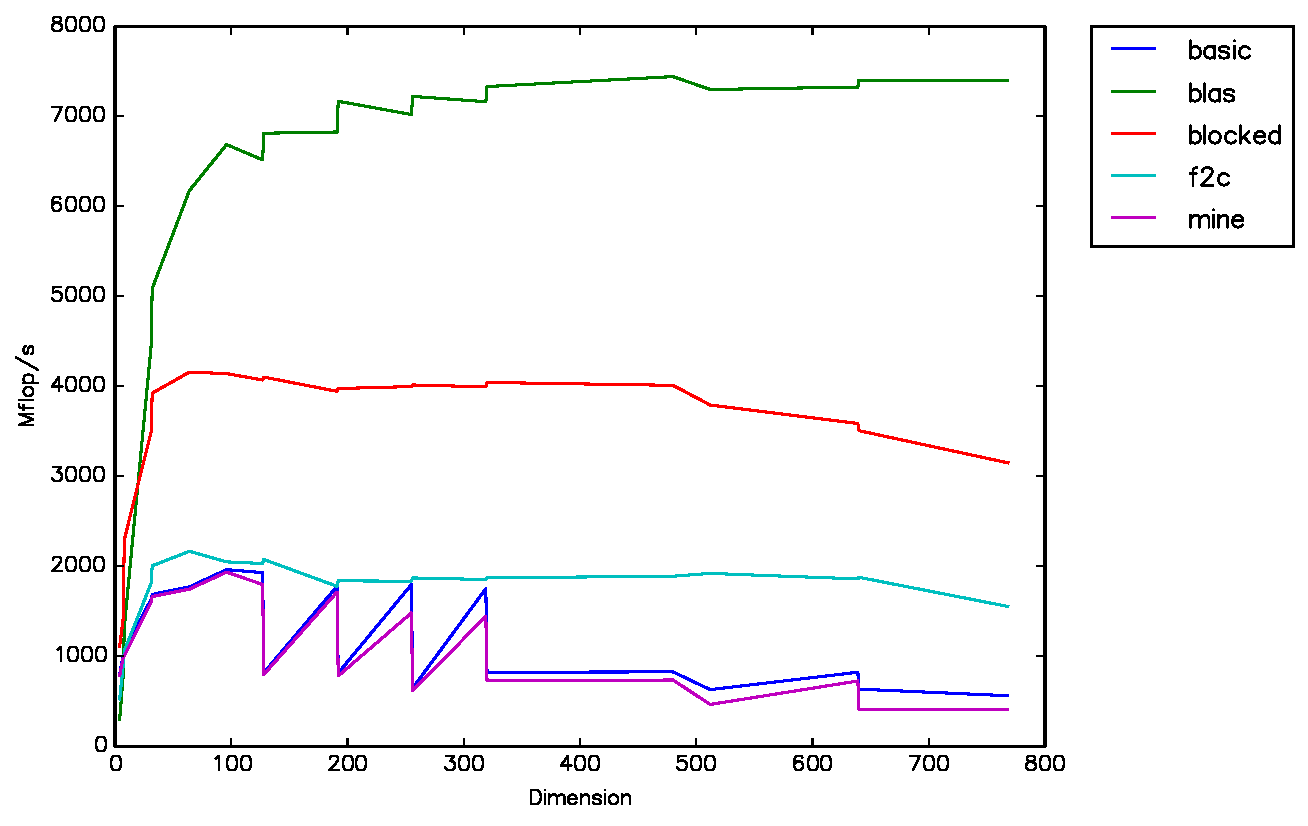
\includegraphics[width=.7\textwidth]{odd.pdf}
    \caption{After adding the odd cases in and using GCC instead of icc(note the ``blocked'' line is ours once again).}
    \label{fig:odd}
  \end{figure}

  The next step to optimizing this was to play with the flags and use tiny code tricks.

  \subsection{Tricks}
    One trick that we played with was to do some loop reordering. In our main block, we have the following

    \begin{lstlisting}
    for (bi = 0; bi < n_blocks; ++bi) {
      const int i = bi * BLOCK_SIZE;
      for (bj = 0; bj < n_blocks; ++bj) {
        const int j = bj * BLOCK_SIZE;
        // trans is our ``transitional'' matrix which contains both At and Bt
        kdgemm2P2(n, tempC, &trans[bi*n*2], &trans[temp + bj*n*2]);
      }
    }
    \end{lstlisting}

    We noted that flipping bi and bj's loop order hurts the performance a lot. For example, at the far end of the spectrum of the sizes
    the different is quite noticable. See table~\ref{tab:looporder}, so we determined that 

    \begin{table}
      \centering
      \begin{tabular}{r c c}
        Size & MFlops (flipped) & MFlops (as shown) \\
        767  & 2660.82 & 3516.27\\
        768  & 2348.95 & 3586.11\\
        769  & 2229.79 & 3503.37
      \end{tabular}
      \caption{Table of loop ordering}
      \label{tab:looporder}
    \end{table}

    Loop reordering was also applied to the copy commands:
    \begin{lstlisting}
    if (odd == 0) {
      for (int j = 0; j<n; j++) {
        for (int i = 0; i < m; i++) {
          At[i*n*2 + 2*j]     = A[j*n + i*2];
          At[i*n*2 + 2*j + 1] = A[j*n + i*2 + 1];
        }
      }
    }
    \end{lstlisting}

    while it wasn't obvious which order should be better as At increments via j via A increments via i, it turns out j, i ordering is \emph{slightly} faster.

    Another small speed increase laid with the serial performance of the copying. Initially, we actually declared to different arrays, one for A and one for B.
    We find that if we just create one giant array of size $2n^2$, and copy A, B into that giant array, performance increase slightly.

    With all these small optimization and the flags (see section below), we achieve performance shown at figure~\ref{fig:final}.

    \begin{figure}[h]
      \centering
      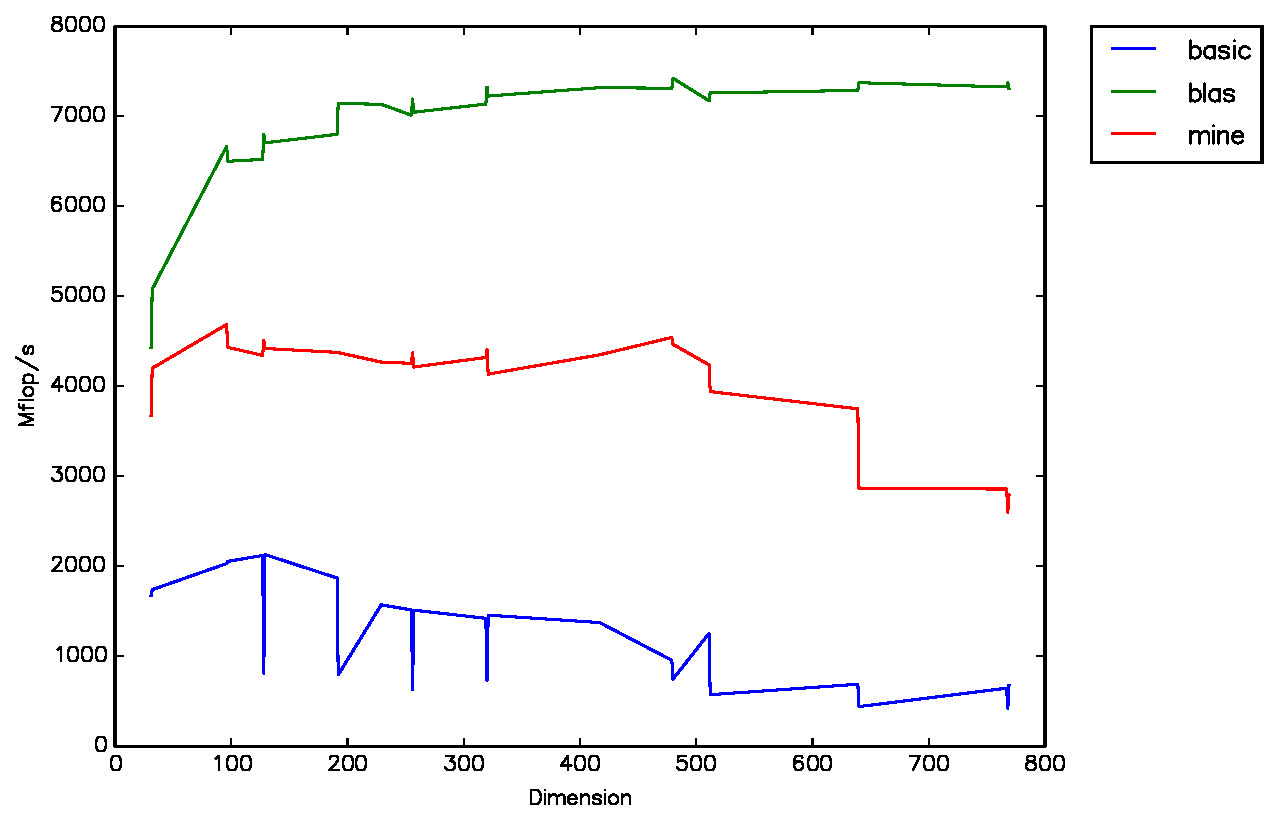
\includegraphics[width=.7\textwidth]{final.pdf}
      \caption{Final speedup}
      \label{fig:final}
    \end{figure}

\section{Compiler Optimization Flags and Keywords}

\subsection{Loop Optimizations}

Since our manual loop unrolling analysis did not significantly improve the performance, we tried the automatic loop unrolling options offered by GCC. We tried each and all combinations of the options mentioned in Table \ref{loop-unrolling}. 

Figure \ref{fig:timing-loops1} shows a comparison between the performance of the Basis configuration and that of each loop optimization flag. \textit{-ftree-loop-im} and \textit{-ftree-loop-linear} do not improve the performance in our case. This was expected for  \textit{-ftree-loop-im} as our code does not have loop invariant code inside loops. Using the \text{-funroll-loops} results in a significant performance improvement because it performs automatic unrolling for some loops that we did not have a chance to unroll manually. 

Figure \ref{fig:timing-loops2} shows a comparison between the \textit{-funroll-loops} flag and all combinations of the loop optimization flags. The combination of \textit{-ftree-loop-im} and \textit{-ftree-loop-linear} more or less has the same performance as that of the Basis configuration. All the other combinations improve the performance significantly and their performances are very close to each other. What is interesting is that \textit{-funroll-loops} is part of all highly performed combinations and its own performance is more or less on par with those combinations. This probably means that most of performance boost is thanks to \textit{-funroll-loops} and other flags have marginal contributions.


\begin{table}
\begin{center}
    \begin{tabular}{ | c | p{10cm} |}
    \hline
    Option & Description \\ \hline
    -ftree-loop-linear  & Applies some linear transformations on loops (reversal, interchange, scaling, and skewing) that may improve cache utilization and simplify the loops to allow other optimizations to take place. In particular, loop interchange may change loop nesting for loops that walk through matrices. \\ \hline
    -funroll-loops &  One of the better known loop transformations. As the name indicates, if the compiler can determine how many iterations will the loop execute, and that number is some small constant N, it emits N copies of the loop body. This may produce faster code at the expense of increased size. \\
    \hline
    -ftree-loop-im & Removes loop invariant code from inside loops. \\ \hline
    \end{tabular}
    \caption{Loop unrolling options that we tried.}
    \label{loop-unrolling}
\end{center}
\end{table}

  \begin{figure}[h]
    \centering
    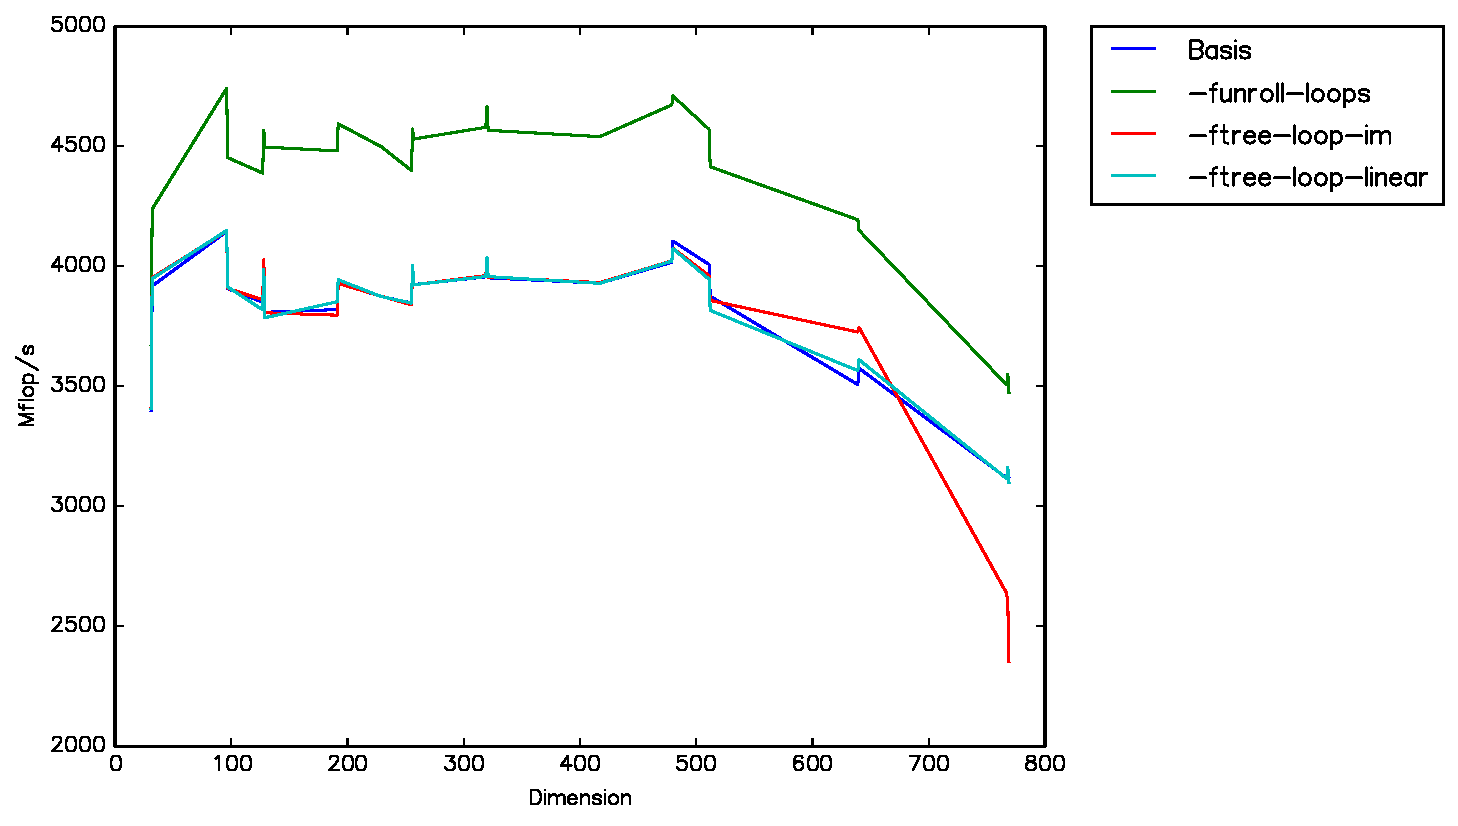
\includegraphics[width=.7\textwidth]{timing-loops-vs-basis.pdf}
    \caption{MFLOPS/s vs Matrix Size: Comparing the basis configuration with each of the loop optimization flags.}
    \label{fig:timing-loops1}
  \end{figure}
  
    \begin{figure}[h]
    \centering
    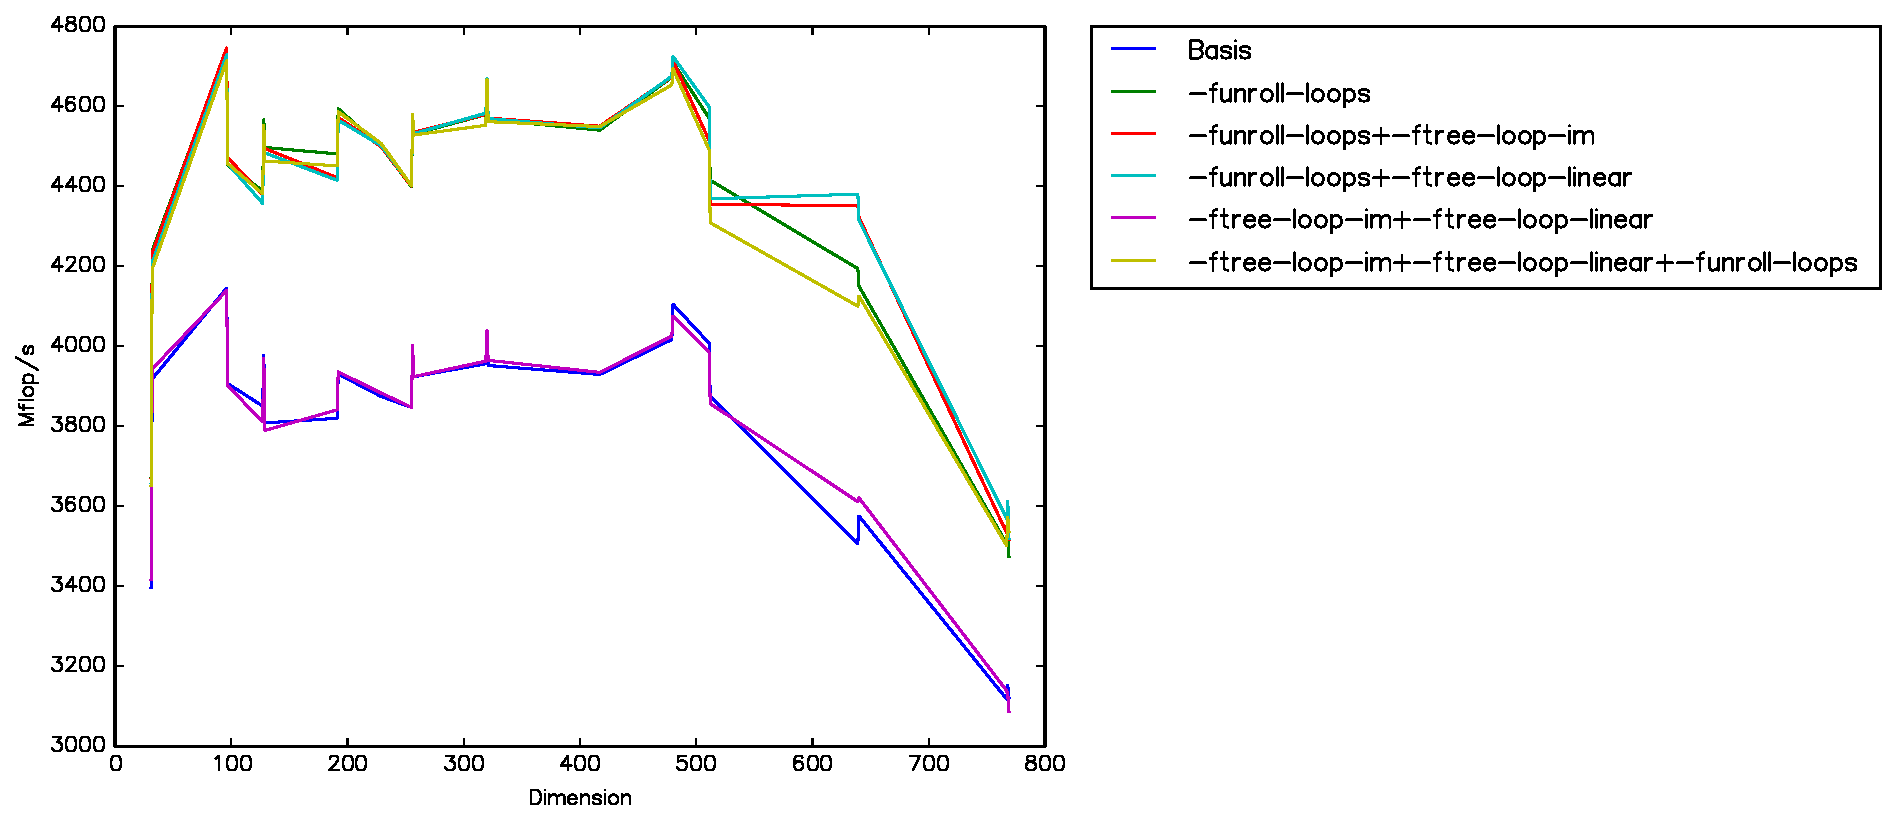
\includegraphics[width=14cm,height=6cm]{timing-loopunroll-vs-combos.pdf}
    \caption{MFLOPS/s vs Matrix Size: Comparing different combinations of loop optimization flags with the Basis configuration and \textit{-funroll-loops}.}
    \label{fig:timing-loops2}
  \end{figure}


\subsection{Restrict Keyword}

The {\bf restrict} keyword is a type qualifier for pointers and is a part of C99 standard. It informs the compiler that the object designated by the pointer cannot be accessed by any other pointer. In other words, the same memory location cannot be pointed to by different pointers. This elimination of memory aliasing helps the compiler to do a better job at loop unrolling.

Since the pointers designating our matrices are non-aliasing, we can declare them as restricted pointers so the compiler can exploit this for automatic unrolling. 
Hence, we tried the restrict keyboard combined with the two loop unrolling options considered in the previous section, i.e. \textit{-funroll-loops} and \textit{-ftree-loops-linear}. 

The outcome can be Fig \ref{fig:restrict}. It turns out that using this keyword not only does not improve the performance but degrades it. The \textit{-funroll-loops} alone without the restrict keyword does a better job that all the combinations considered here. Hence, we will not consider this flag in our analysis for finding the optimal combination of optimization flags.


    \begin{figure}[h]
    \centering
    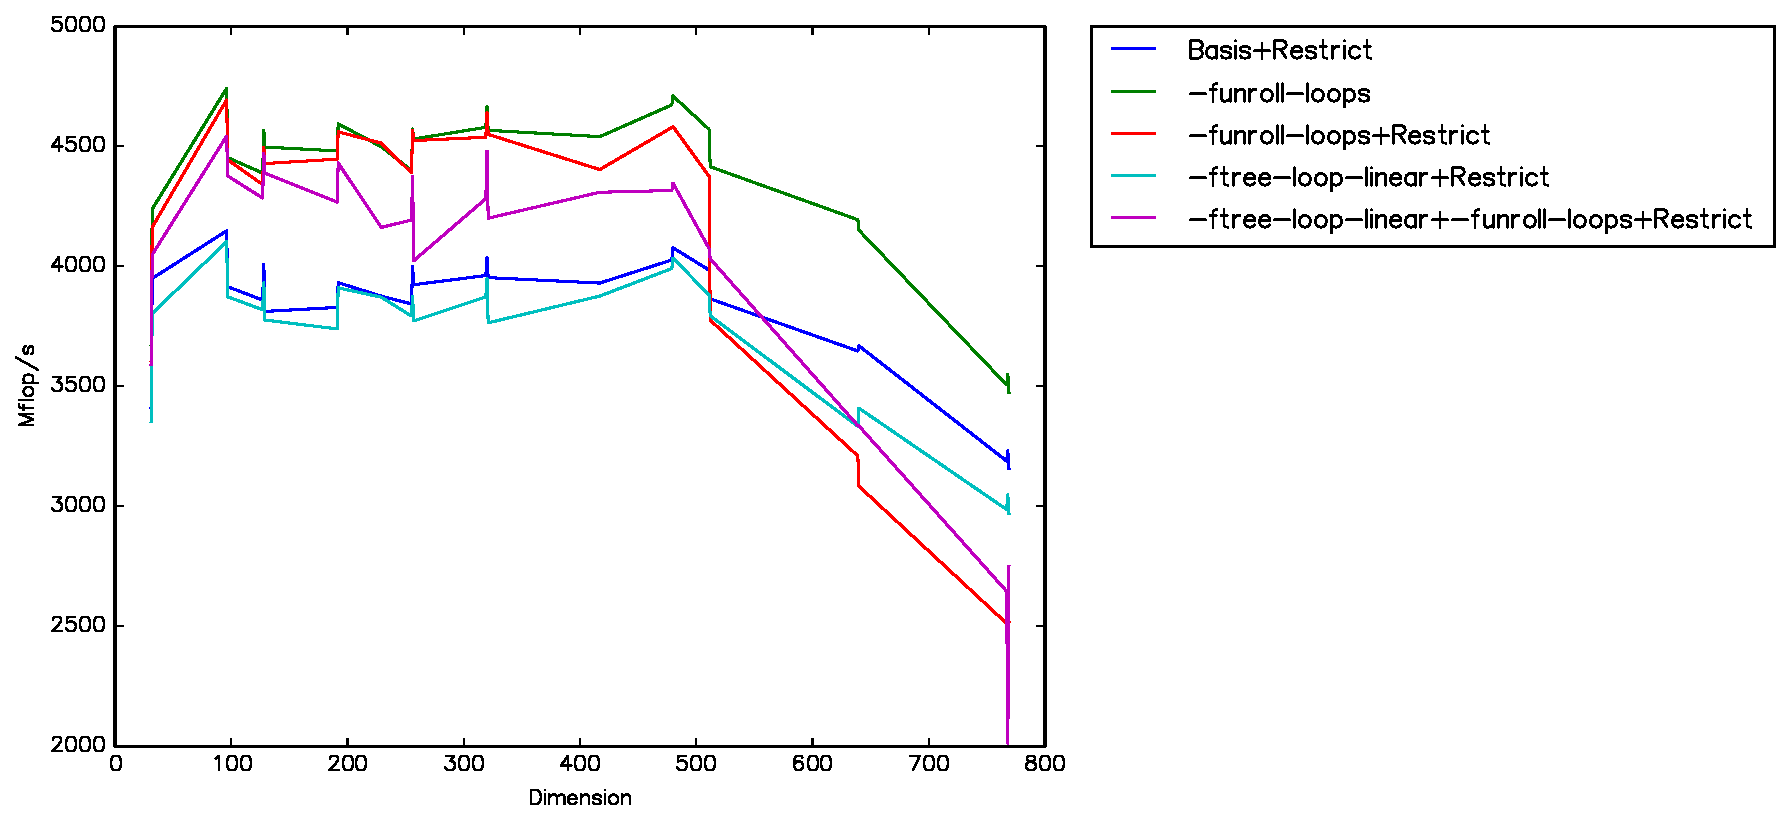
\includegraphics[width=14cm,height=6cm]{timing-loops-restrict.pdf}
    \caption{MFLOPS/s vs Matrix Size: Different combinations of loop unrolling flags with the restrict keyword.}
    \label{fig:restrict}
  \end{figure}

\subsection{Fast Floating Point Operations}

The \textit{-ffast-math} option includes most of GCC flags for fast floating point arithmetic optimization.  This option is not always recommended though because it breaks strict IEEE compliance on floating-point operations which might result in accumulation of computational errors of unpredictable nature. Since the accuracy of our matrix multiplication routine is verified within the \textit{ matmul.c} function, we decided to give \textit{-ffast-math} a try. As can be seen in Fig \ref{fig:timing-math}, this option does not affect the performance significantly and indeed it degrades the performance for some cell sizes. Hence, we will not consider this flag in our analysis for finding the optimal combination of optimization flags.
 

  \begin{figure}[h]
    \centering
    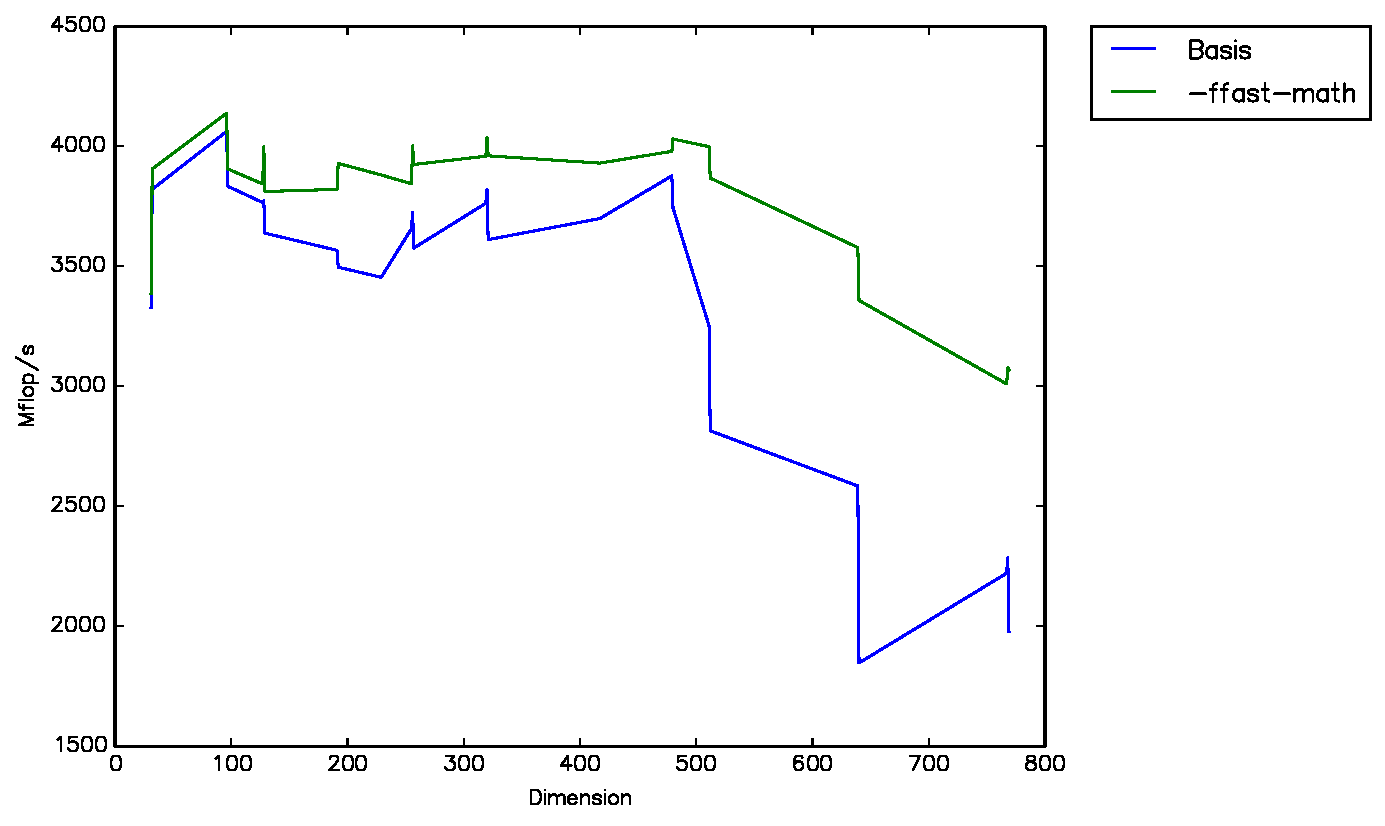
\includegraphics[width=.7\textwidth]{timing-math.pdf}
    \caption{MFLOPS/s vs Matrix Size for \textit{-ffast-math}.}
    \label{fig:timing-math}
  \end{figure}

\subsection{Architecture Specific Flags}

Different CPUs have different capabilities, support different instruction sets, and have different ways of executing code. \textit{-march} and \textit{-mtune} are the most common GCC flags for this purpose. On \textit{x86} and \text{x86-64} CPUs, which includes the Xeon E5504 cores on our instructional nodes, \textit{-march} will generate code specifically for that CPU using all its available instruction sets and the correct ABI. Also, including \textit{-march} implies \textit{-mtune}. So, unless we are not aware of the processor family we are using, having \textit{-mtune} must be enough. 

We have GCC 4.8.2 on the cluster. The relevant \textit{-mtune} options on this version that are relevant to our processor are described in Table \ref{tab:arch-march}. Our processor, Xeon E5504, has the Nehalem-EP microarchitecture. The newer Intel Corei7 processors are mostly based on this architecture. That is why \textit{corei7} seems to be the most relevant option. However, GCC is not that consistent about how it treats architecture specific flags. That is why we also considered the \textit{core2} and \textit{native} options. The reason for \textit{core2} is that Nehalem-EP is a successor of the Core microstructure and we considered \textit{native} because it lets the compiler to determine the architecture by itself. 

Figure \ref{fig:timing-march} shows the performance obtained by each case compared to the basis configuration.The three options do not significantly affect the performance, although \textit{native} seems to perform better for larger sizes. This is probably because our kernel is already an SSE code and hence is not affected much by architecture specific flags. 

Although the architecture specific flags do not seem to improve the performance by themselves, they might do so in combination with other flags as they might change the way the compiler use certain flags. Hence, we will reconsider these flags in our analysis for finding the optimal combination of optimization flags.

\begin{table}
\begin{center}
    \begin{tabular}{ | c | p{10cm} |}
    \hline
    Option & Description \\ \hline
    Native  & This selects the CPU to tune for at compilation time by determining the processor type of the compiling machine. Using -mtune=native will produce code optimized for the local machine under the constraints of the selected instruction set. Using -march=native will enable all instruction subsets supported by the local machine (hence the result might not run on different machines).  \\ \hline
    corei7 & Intel Core i7 CPU with 64-bit extensions, MMX, SSE, SSE2, SSE3, SSSE3, SSE4.1 and SSE4.2 instruction set support. \\ \hline
    core2 & Intel Core 2 CPU with 64-bit extensions, MMX, SSE, SSE2, SSE3 and SSSE3 instruction set support. \\ \hline
    \end{tabular}
    \caption{Loop unrolling options that we tried.}
    \label{tab:arch-march}
\end{center}
\end{table}


  \begin{figure}[h]
    \centering
    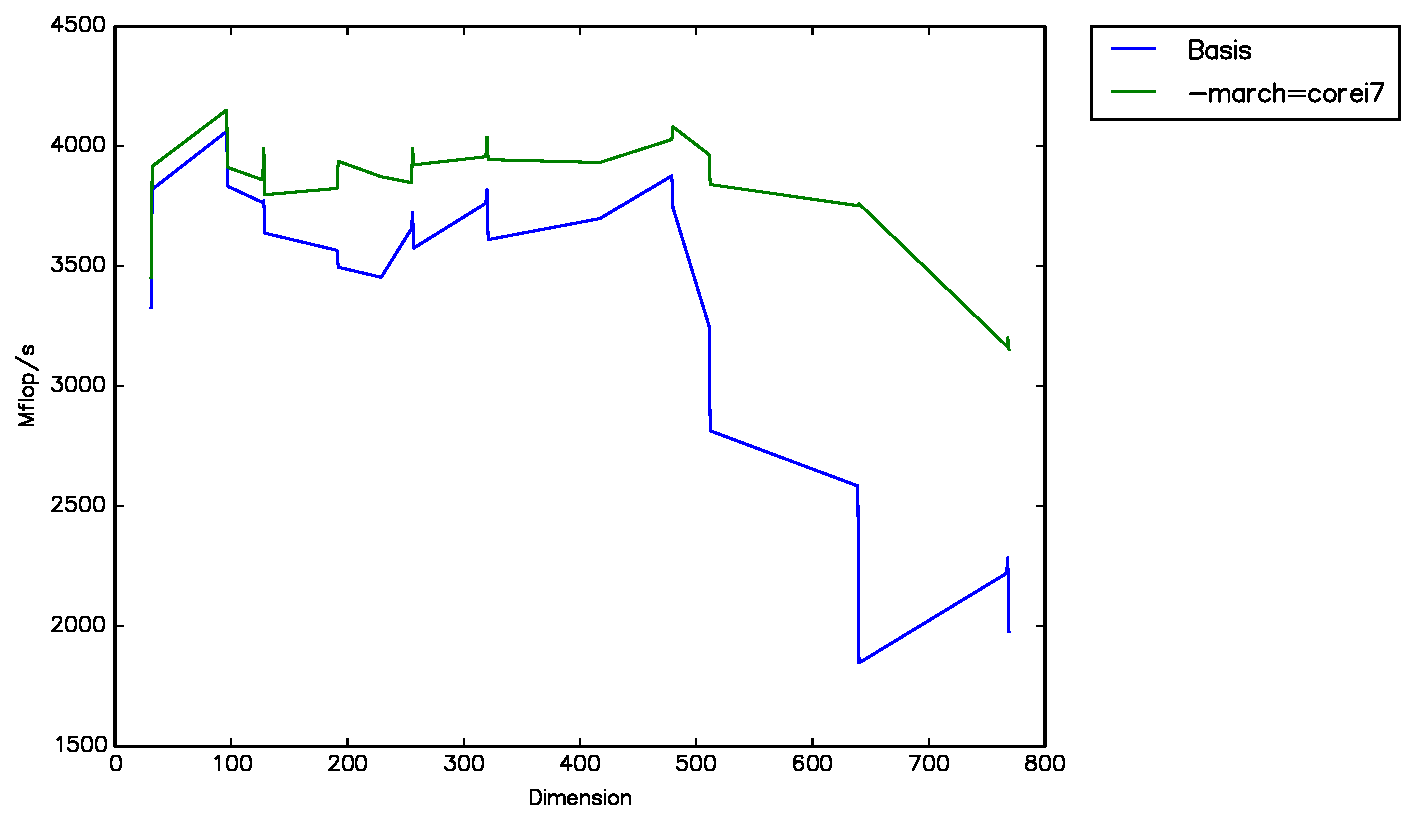
\includegraphics[width=.7\textwidth]{timing-march.pdf}
    \caption{MFLOPS/s vs Matrix Size for \textit{-march=corei7}.}
    \label{fig:timing-march}
  \end{figure}
 
\subsection{Combining Flags}

We start our analysis by considering all combinations of those flags that that either improved the performance in our observations or could potentially do so by being combined with other flags. For the loop optimization flags, we chose the 4 combinations that involved \textit{-funroll-loops} in them as they all improved the performance at a similar level, c.f. Fig \ref{fig:timing-loops2}. As for architecture specific flags, we only considered \textit{-march = native} because, as shown in Fig \ref{fig:timing-march}, the three flags result in more or less the same performance.  Therefore, the combinations we considered were the following:

\begin{enumerate}

\item OPTFLAGS = -O3 -msse4.2 -ftree-loop-linear -funroll-loops -ftree-loop-im -march=native

\item OPTFLAGS = -O3 -msse4.2 -ftree-loop-linear -funroll-loops -march=native

\item OPTFLAGS = -O3 -msse4.2 -ftree-loop-im -funroll-loops -march=native

\item OPTFLAGS = -O3 -msse4.2 -funroll-loops -march=native

\item OPTFLAGS = -O3 -msse4.2 -funroll-loops

\end{enumerate}

Note that \textit{O3} and \textit{-msse4.2} constitute our Basis configuration which all the other include. The reason for \textit{O3} is that our observations showed that, when used with the above flags, it results in better performance than \textit{O1} and \textit{O2}. We used \textit{-msse4.2} in our Basis configuration because it is the fastest SSE flag for our architecture. 

 
Fig \ref{fig:combo-analysis1} shows the the outcome for all of the above combinations. The 3rd, 4th and 5th combinations clearly do a better job. Their outcomes are shown in Fig \ref{fig:combo-analysis2}. It can be seen that the 3rd  and 4th combinations perform slightly better and have more or less the same performance. The better performance of these combinations compared to the 5th one is thanks to the architecture specific flag \textit{-march = native} because, as mentioned in the Loop Optimization section, the \textit{-ftree-loops-im} flag has a significantly smaller contribution compared to \textit{-funroll-loops}. Hence, we pick the 4th combination namely

\begin{itemize}

\item OPTFLAGS = -O3 -msse4.2 -funroll-loops -march=native

\end{itemize}

as our optimal configuration of compiler optimization flags. Fig \ref{fig:final-vs-blas} shows the performance of our code in comparison with those of Blas and the native code under the same configuration.
 
  \begin{figure}[h]
    \centering
    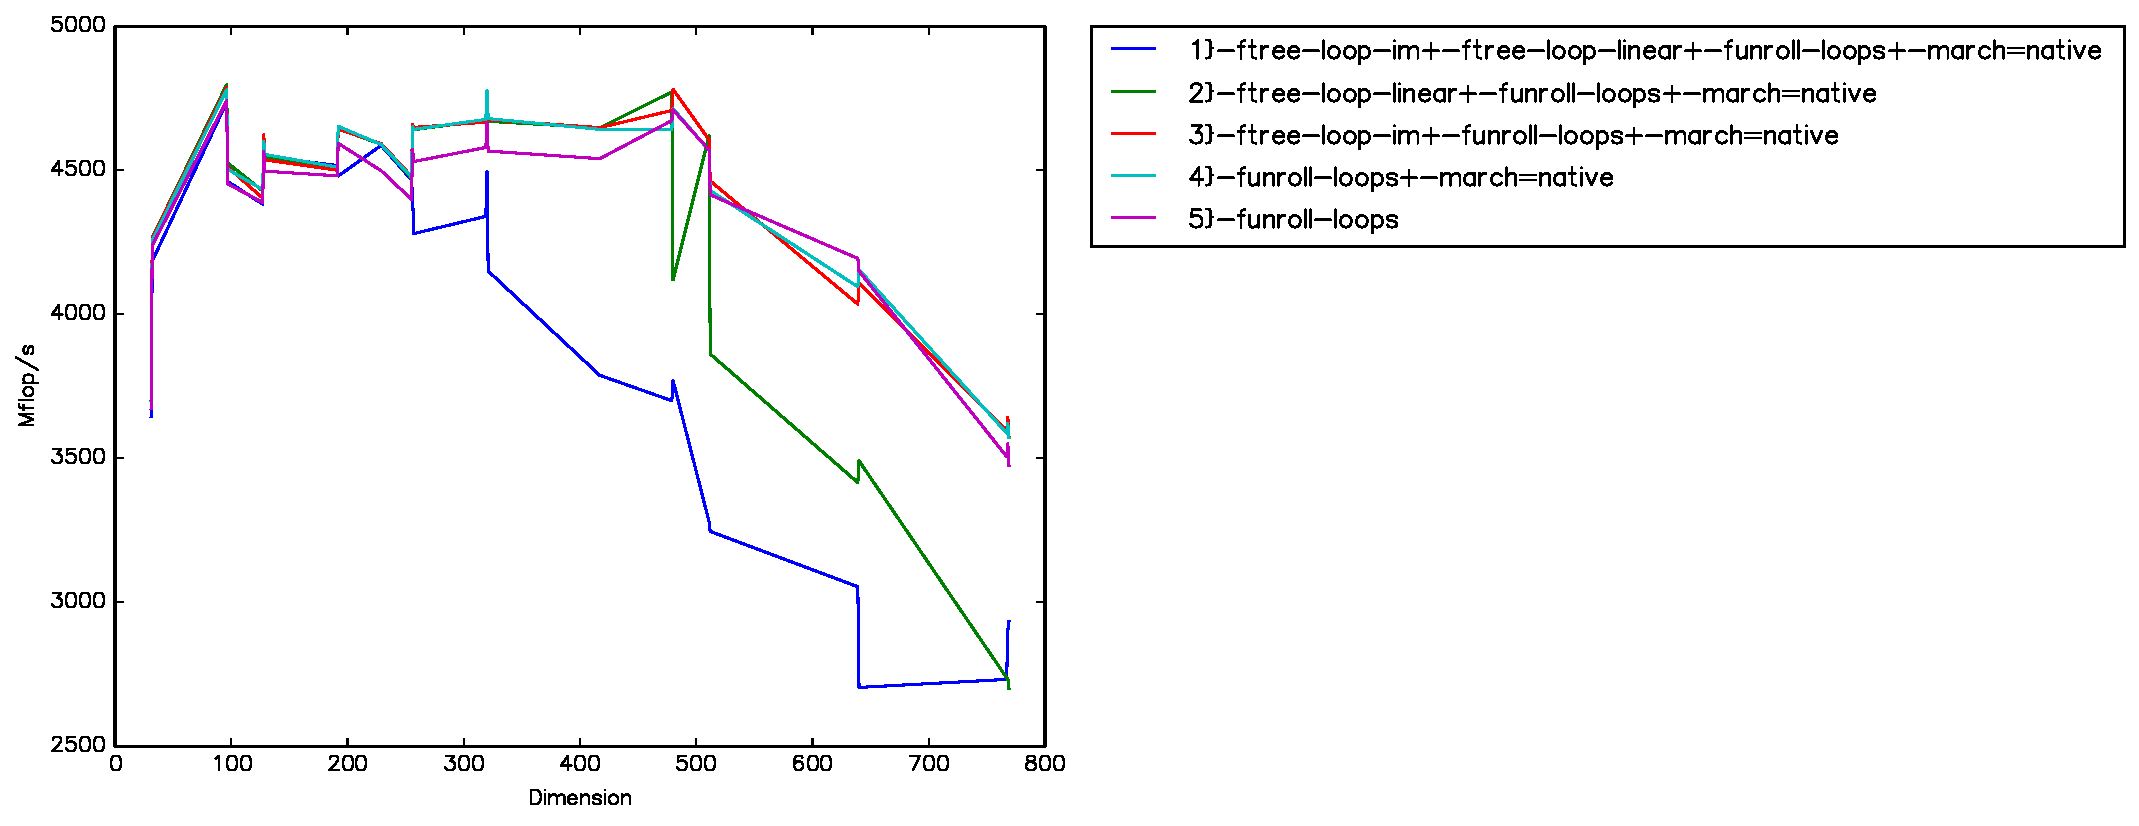
\includegraphics[width=16cm,height=7cm]{timing-final-config.pdf}
    \caption{MFLOPS/s vs Matrix Size: combinations considered for finding the optimal configuration of the compiler optimization flags.}
    \label{fig:combo-analysis1}
  \end{figure}

  \begin{figure}[h]
    \centering
    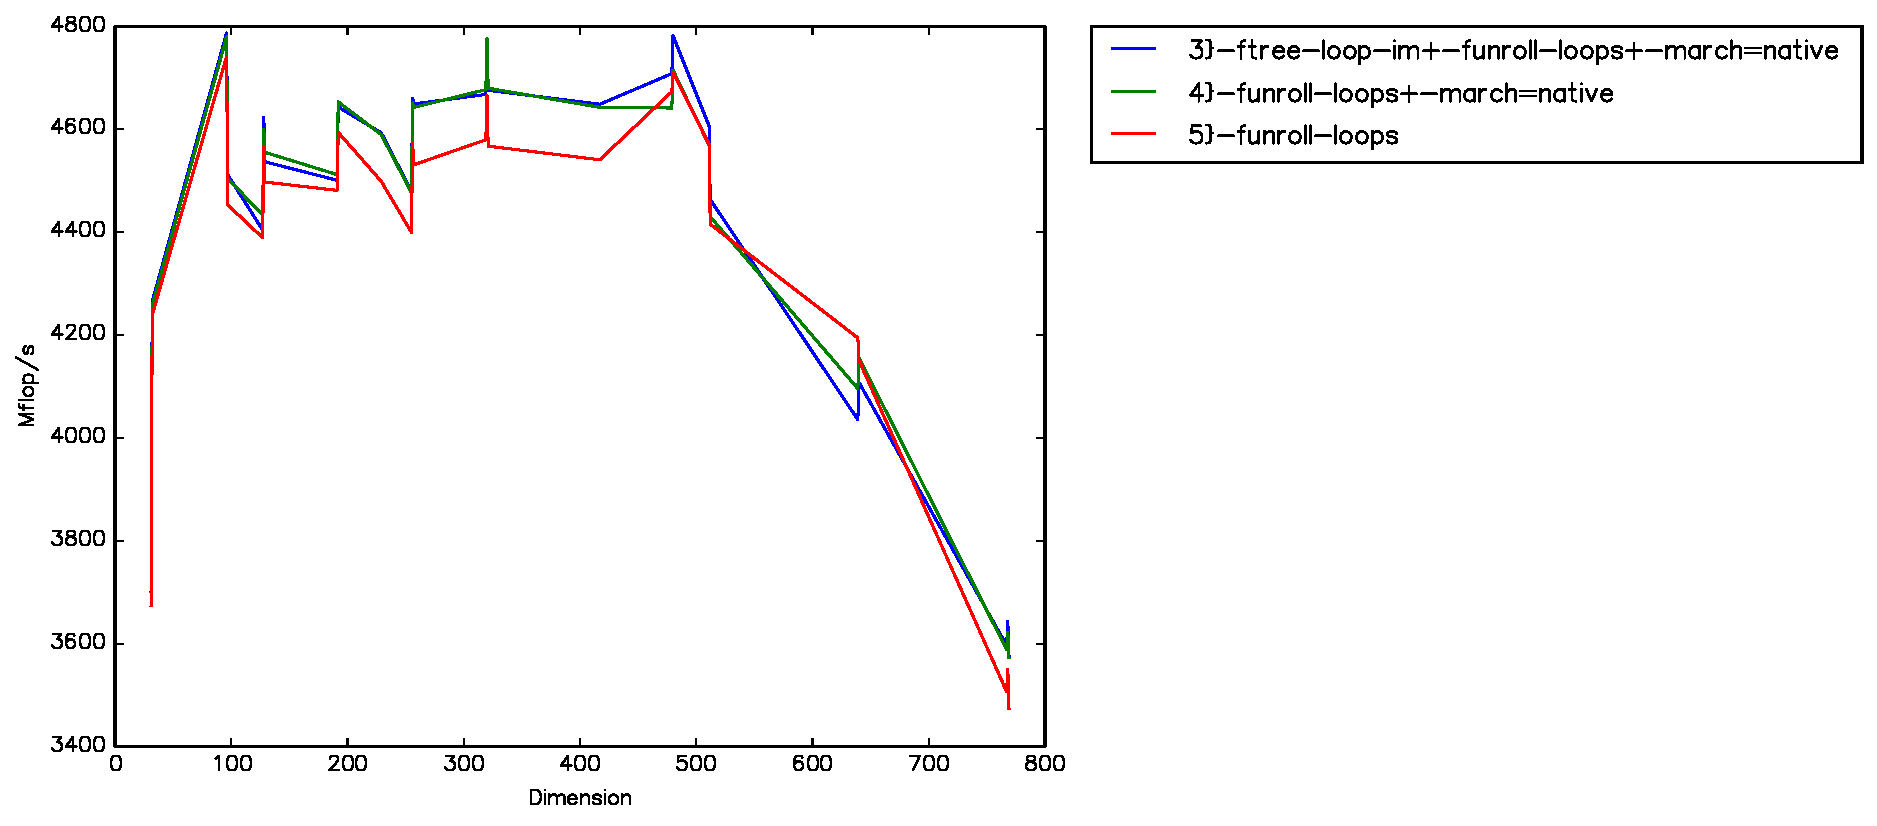
\includegraphics[width=16cm,height=7cm]{timing-final-config-clear.pdf}
    \caption{MFLOPS/s vs Matrix Size: the three combinations that performed better in our analysis on the compiler optimization flags.}
    \label{fig:combo-analysis2}
  \end{figure}
  
    \begin{figure}[h]
    \centering
    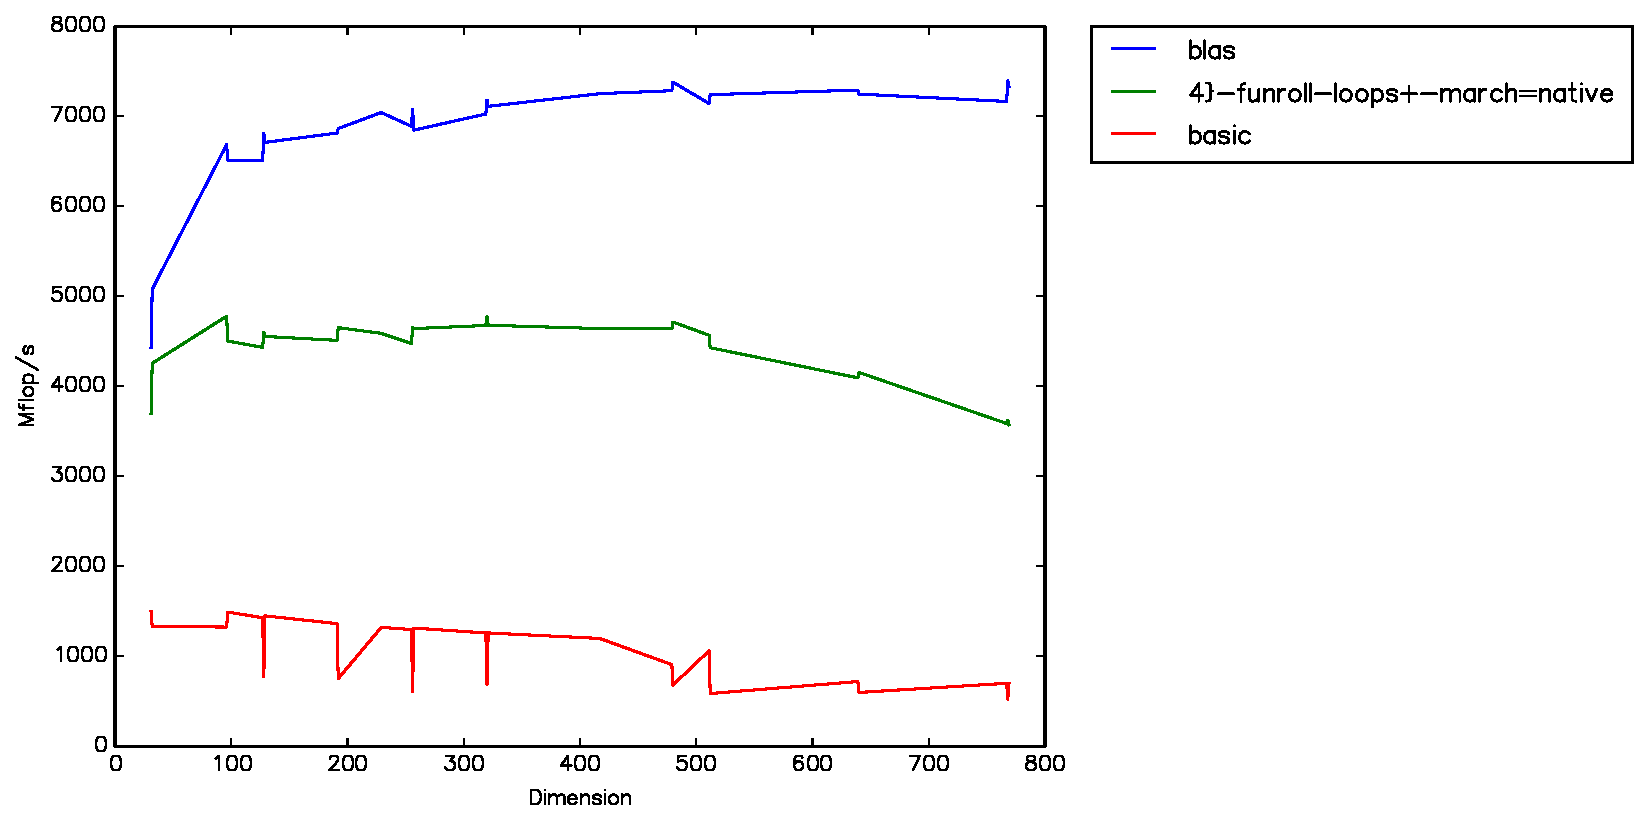
\includegraphics[width=16cm,height=7cm]{timing-final-vs-blas.pdf}
    \caption{MFLOPS/s vs Matrix Size: the final optimized code vs Blas and the naive code.}
    \label{fig:final-vs-blas}
  \end{figure}

    \subsection{Memory Usage}

    One thing we tried was to break up the P by 2 and 2 by P matrices into smaller block. Theoretically, since the size of a double is 8 bytes, we need to fit
    $2(2P)*8 + 4 = 32P + 4$ bytes into the cache. While the level 1 cache of the educational nodes are quite low, it seems to not matter from the plots (our maximum
    size that we can fit in the L1 cache is $P=128$). If we look at the level 2 cache, our array size can go up to 1024 theoretically, which (theoretically) shouldn't
    impede us.

    If we look at the cachegrind output for our program, we see the following:
    \begin{lstlisting}
[sj423@en-cluster02 matmul]$ valgrind --tool=cachegrind ./matmul-blocked
==18730== Cachegrind, a cache and branch-prediction profiler
==18730== Copyright (C) 2002-2013, and GNU GPL'd, by Nicholas Nethercote et al.
==18730== Using Valgrind-3.9.0 and LibVEX; rerun with -h for copyright info
==18730== Command: ./matmul-blocked
==18730== 
--18730-- warning: L3 cache found, using its data for the LL simulation.
--18730-- warning: pretending that LL cache has associativity 24 instead of actual 16
Compiler:	gcc
Options:	-O3 -funroll-loops -msse4.2 -ffast-math -mtune=generic -march=corei7
Description:	Simple blocked dgemm.

==18730== 
==18730== I   refs:      62,147,347,847
==18730== I1  misses:             1,539
==18730== LLi misses:             1,518
==18730== I1  miss rate:           0.00%
==18730== LLi miss rate:           0.00%
==18730== 
==18730== D   refs:      32,109,636,396  (27,962,135,435 rd   + 4,147,500,961 wr)
==18730== D1  misses:     1,976,702,658  ( 1,966,158,637 rd   +    10,544,021 wr)
==18730== LLd misses:         7,256,578  (     5,016,816 rd   +     2,239,762 wr)
==18730== D1  miss rate:            6.1% (           7.0%     +           0.2%  )
==18730== LLd miss rate:            0.0% (           0.0%     +           0.0%  )
==18730== 
==18730== LL refs:        1,976,704,197  ( 1,966,160,176 rd   +    10,544,021 wr)
==18730== LL misses:          7,258,096  (     5,018,334 rd   +     2,239,762 wr)
==18730== LL miss rate:             0.0% (           0.0%     +           0.0%  )
    \end{lstlisting}

    which actually mimics the performance of the BLAS cache stats:

    \begin{lstlisting}
[sj423@en-cluster02 matmul]$ valgrind --tool=cachegrind ./matmul-blas 
==1449== Cachegrind, a cache and branch-prediction profiler
==1449== Copyright (C) 2002-2013, and GNU GPL'd, by Nicholas Nethercote et al.
==1449== Using Valgrind-3.9.0 and LibVEX; rerun with -h for copyright info
==1449== Command: ./matmul-blas
==1449== 
--1449-- warning: L3 cache found, using its data for the LL simulation.
--1449-- warning: pretending that LL cache has associativity 24 instead of actual 16
Compiler:	gcc
Options:	-O3 -funroll-loops -msse4.2 -ffast-math -mtune=generic -march=corei7
Description:	System CBLAS dgemm.

==1449== 
==1449== I   refs:      59,157,389,231
==1449== I1  misses:             2,399
==1449== LLi misses:             2,297
==1449== I1  miss rate:           0.00%
==1449== LLi miss rate:           0.00%
==1449== 
==1449== D   refs:      30,847,547,276  (26,700,497,225 rd   + 4,147,050,051 wr)
==1449== D1  misses:     1,670,642,244  ( 1,665,753,557 rd   +     4,888,687 wr)
==1449== LLd misses:         3,023,479  (     2,584,556 rd   +       438,923 wr)
==1449== D1  miss rate:            5.4% (           6.2%     +           0.1%  )
==1449== LLd miss rate:            0.0% (           0.0%     +           0.0%  )
==1449== 
==1449== LL refs:        1,670,644,643  ( 1,665,755,956 rd   +     4,888,687 wr)
==1449== LL misses:          3,025,776  (     2,586,853 rd   +       438,923 wr)
==1449== LL miss rate:             0.0% (           0.0%     +           0.0%  )
    \end{lstlisting}

    Note that it's a similar miss rate in terms of percentages, but our algorithm had to
    use much more read/writes than the BLAS algorithm, which contributes to inefficiencies.

    It's quite interesting to see that such small differences in the miss rates will result in such a large cut in performance
    from the BLAS package.

    \subsection{New Kernel}

While benchmarking matrix multiplication based on Bindel's kernel we also attempted to write a faster one, 
focusing on multiplying 8x8 matrices (saved in mm\_kernel/kdgemm\_doublerainbow.c). The approach was fairly straightforward: starting with a 
naive implementation we unrolled the 2 inner loops and replaced adjacent operations with their equivalent SSE instructions. 
Afterwards it became clear that replacing A and C with their transposes would make all memory accesses to each matrix sequential,
improving cache use. This put the kernel on par with Bindel's.
\begin{table}[h]
  \centering
  \begin{tabular}{r c c}
    Name & Size & MFlops\\
    Our (double rainbow) & 8 by 8 by 8 & 5525.91 \\
    Bindel's 2P2 (gcc) & 2 by 5000 by 2 & 4885.36 \\
    Our (double rainbow 4 x 4) & 4 by 4 by 4 & 4178.78 \\
    Bindel's 2P2 (icc) & 2 by 5000 by 2 & 3644.69 \\
    Naive (simple) & 4 by 4 by 4& 2964.03
  \end{tabular}
  \caption{Kernel Timing Results (Note: Bindel's kernel seems to do slightly better for larger $P$ values).}
  \label{tab:kernel}
\end{table}
Several other optimizations were tried to no benefit. 
Unlike Bindel's kernel the basic 8x8 SSE is faster with the Intel compiler than gcc. 
After reading some documentation on icc we found a flag called 'fast' that makes architecture-specific optimizations 
and added the equivalent flags for the cluster nodes, but this didn't help. There was no gain from adding more temporary variables
to eliminate false dependencies past the 8 in the final version. We also tried reducing the matrix size to 4x4 which actually resulted in a performance decrease.

We eventually did luck into another performance boost. Using Bindel's kernel we had experimented with the -funroll-loops
flag and assumed it would do a near optimal job, and thought this would be especially true on a small matrix with size known at compile time.
This turned out to be wrong. After adding '\#pragma unroll(8)' above the main loop on a whim the kernel jumped to 5500Mflops (see table~\ref{tab:kernel}).
The use of icc compiler actually was better for our kernel, compared to Dr. Bindel's.

The new kernel was not ready in time to integrate with the main dgemm routine. It is available only in mm\_kernel/kdgemm\_doublerainbow.c. 
It is likely some performance would be lost making it work with larger matrices. One thing to note though was that using Dr. Bindel's
kernel, we achieved roughly 4 Gflops of performance, while the simplest case in ktimer allowed 4.8 Gflops. One can safely hypothesize that
with an 8 by 8 kernel, we would get about 5 Gflops in performance for the best cases, and slightly lower for odd cases.
\end{document}
